This section aims to dive into the fascinating history and evolution of Bitcoin mining equipment, tracing its origins from the early days of Bitcoin to its present-days. The focus will be especially onto the technologies that have transformed, year after year, Bitcoin mining into a globally recognized industry.

\noindent As already said, the first block was mined by Satoshi Nakamoto on January 3, 2009. At the beginning of Bitcoin, the network difficulty was 1. Since there was very little people who was mining in the first days, the difficulty didn't increased, and so it was possible to mine Bitcoin blocks using an average personal computer. In fact, it was the unique time in which only a Central Processing Unit (\textbf{CPU}) was enough to mine bitcoin. As the potential reward for mining received more media attention, especially after the historical first-ever real-world transaction using bitcoin where the programmer named Laszlo Hanyecz spent 10000 bitcoin on two Papa John's pizzas (May 18, 2010 \cite{bitcoinpizzas}), the mining difficulty started to rise.\\
In \textbf{October 2010}, the first mining device based on Graphics Processing Units (\textbf{GPU}s) was developed. As clearly represented in \ref{fig:bitcoin_mining_history}, thanks to GPU's excellence at computing simple mathematical operations in parallel, GPUs hugely increased the global hashrate, leading to a network difficulty increase.
\begin{figure}[h!]
\centering
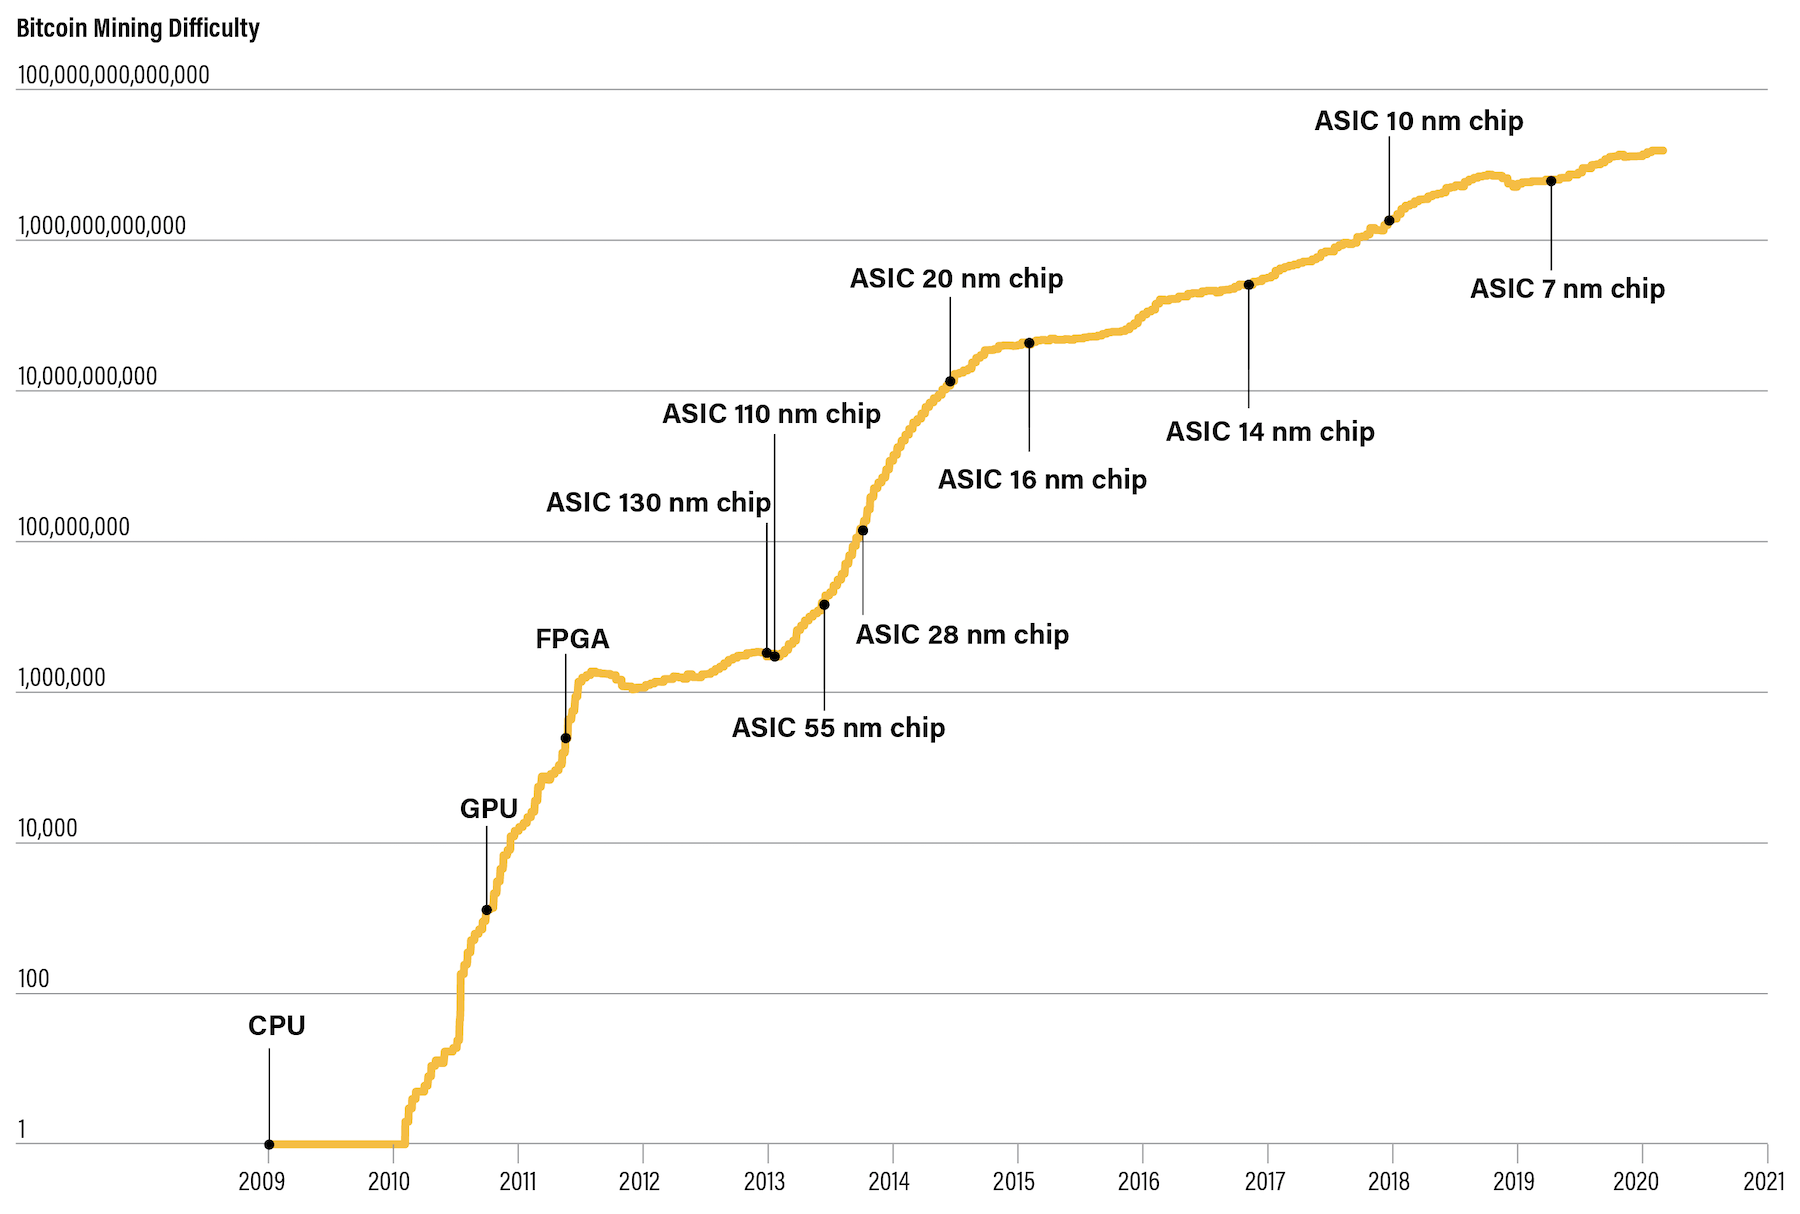
\includegraphics[width=14.5cm]{Figures/mining/mining-evolution.png}
\caption{Bitcoin mining hardware evolution, in relation to the network difficulty}
\label{fig:bitcoin_mining_history}
\end{figure}
\newpage
\noindent During the following year, \textbf{2011}, the Field Programmable Gate Arrays (\textbf{FPGA}) came into the mining game. They were even faster than GPUs in term of hashing power, contributing to the ever-increasing network hashrate, and difficulty.\\
The third major advancement in Bitcoin mining required an extensive allocation of resources, time, and development efforts. The focus during those years was on creating a completely novel machine solely specialized to Bitcoin mining. The hard work in research \& development got the first results in \textbf{2013},  when the Chinese company called Canaan Creative, introduced the first set of Application-Specific Integrated Circuits (\textbf{ASIC}s) designed exclusively for Bitcoin mining.\\
In contrast to CPUs, GPUs, and FPGAs, these ASIC devices were specifically built with the intention of being used exclusively for Bitcoin mining. This included pre-designing and optimizing all hardware and software components of these ASIC devices to efficiently compute the precise calculations required for generating new Bitcoin blocks. While Canaan Creative emerged as the inaugural Bitcoin ASIC manufacturer, other players like Bitmain and MicroBT also joined the game, introducing their own models of ASIC mining devices with increasingly advanced hardware. A significant evolution in ASIC mining technology since 2013 has been the consistent reduction in chip size. Beginning at a size of 130nm in 2013, the ASIC chips have undergone remarkable shrinkage, with the latest hardware models featuring diminutive sizes as small as 5nm. The transistor size reduction led to an increasing efficiency in ASIC machines. Nowadays, an ASIC bitcoin mining device is estimated to be 100 billion times more efficient than the average CPU back in 2009. 
\begin{figure}[h!]
\centering
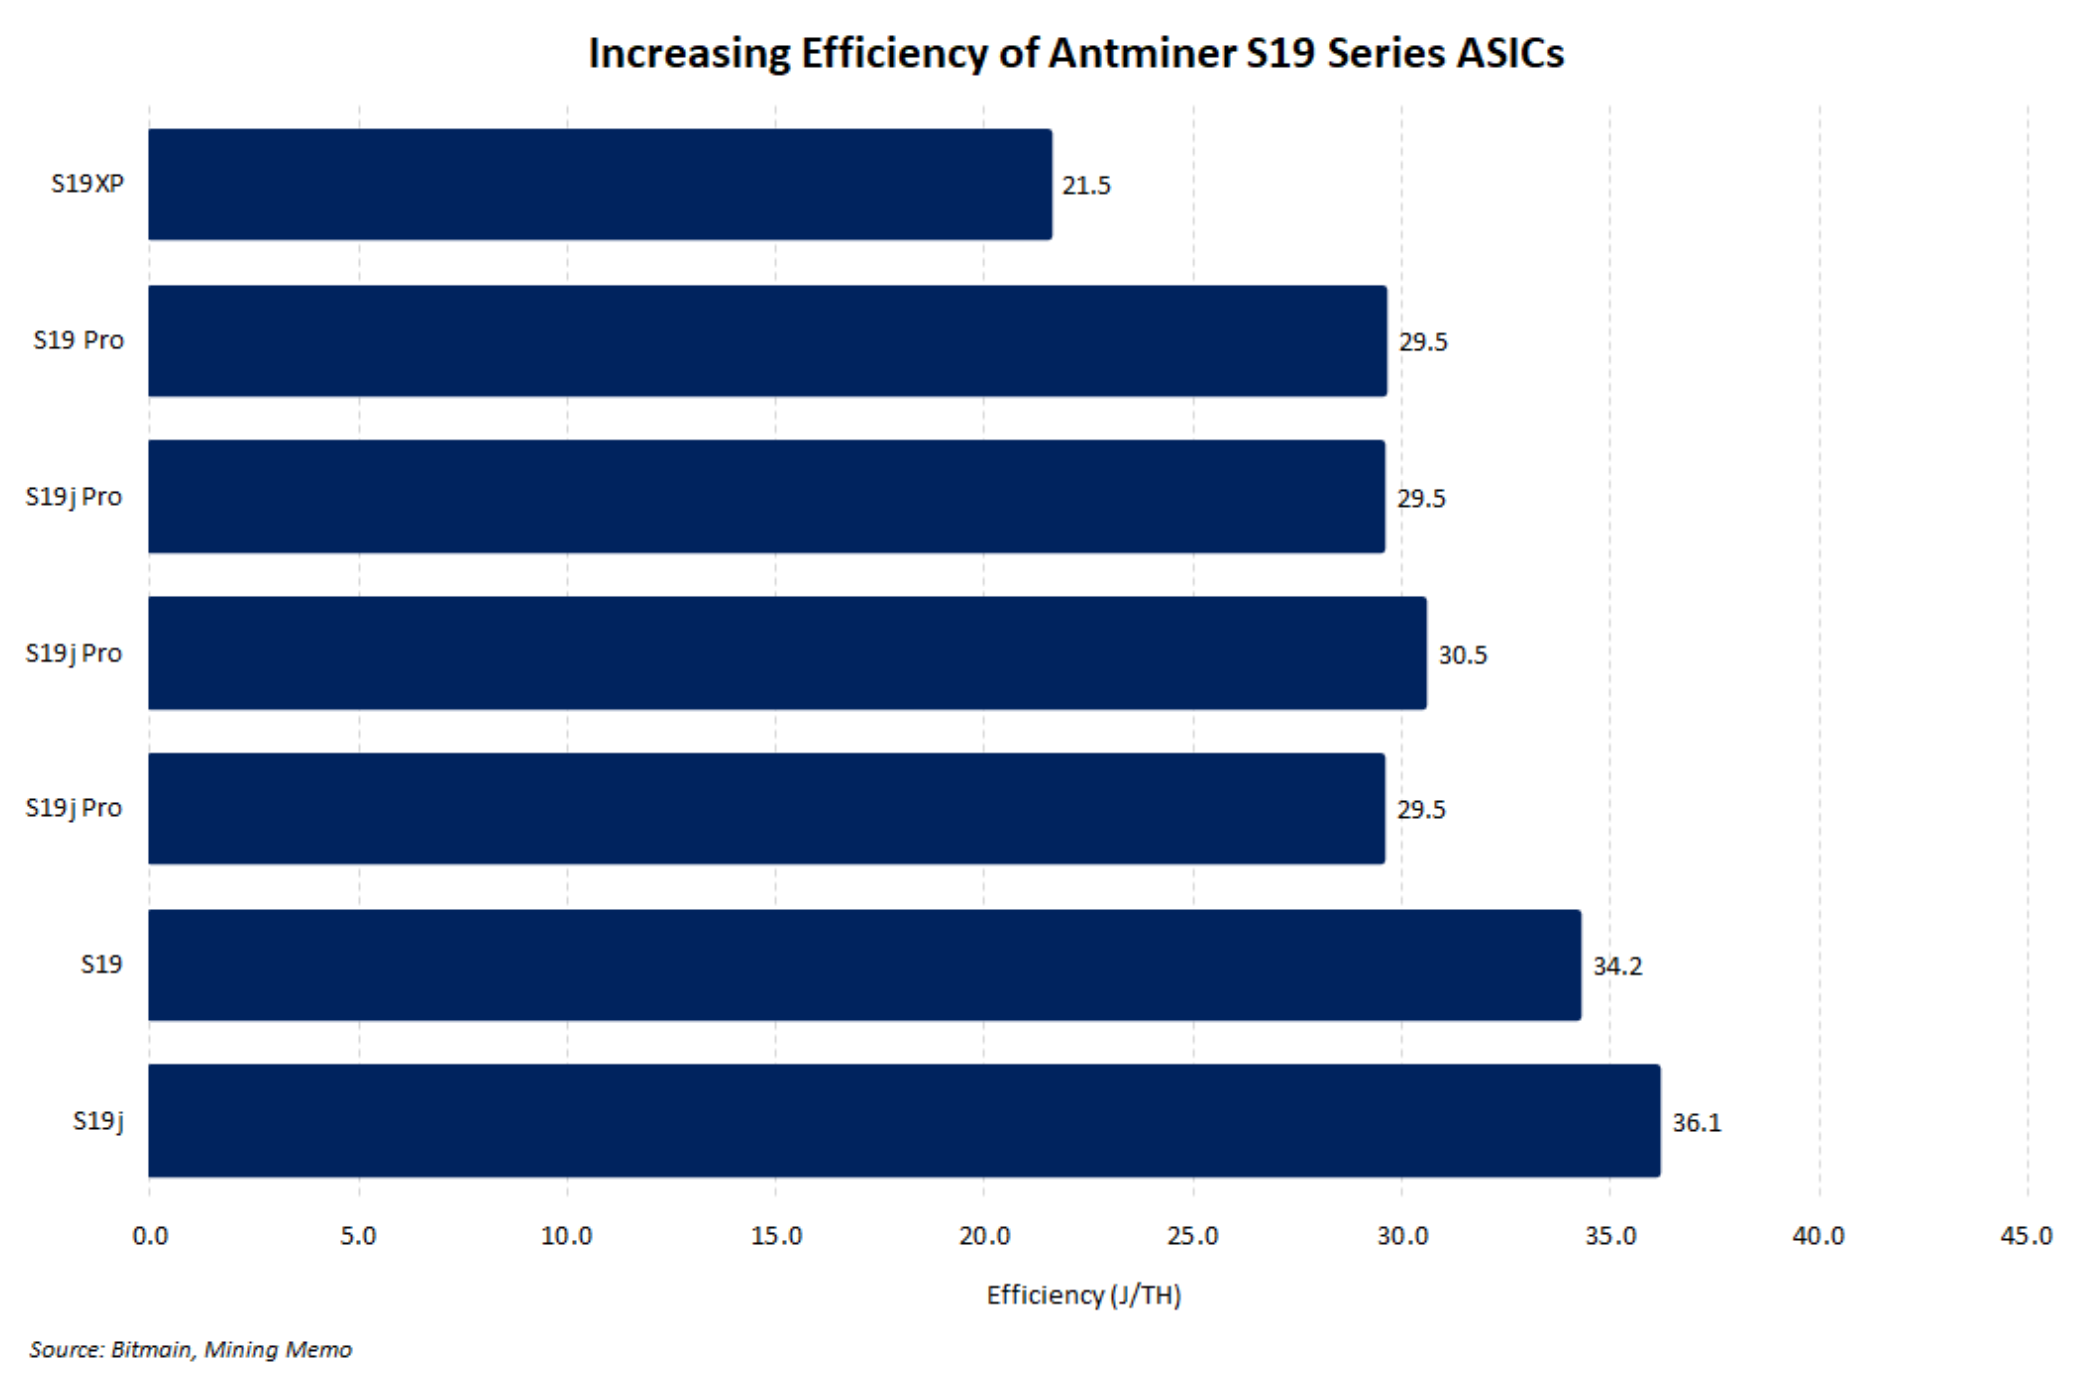
\includegraphics[width=12.5cm]{Figures/mining/s19-efficiency.png}
\caption{Antminer S19 model series, with relative efficiency (J/TH)}
\label{fig:s19-efficiency}
\end{figure}